\section{Methodology}

\begin{frame}{Chain-of-Thought Prompting}
    \textit{Chain-of-Thought} (CoT) prompting~\cite{wei2023chainofthought}, which uses a series of intermediate reasoning steps, significantly improves the ability of LLMs to perform complex reasoning.\\
    \begin{figure}[!htb]
        \centering
        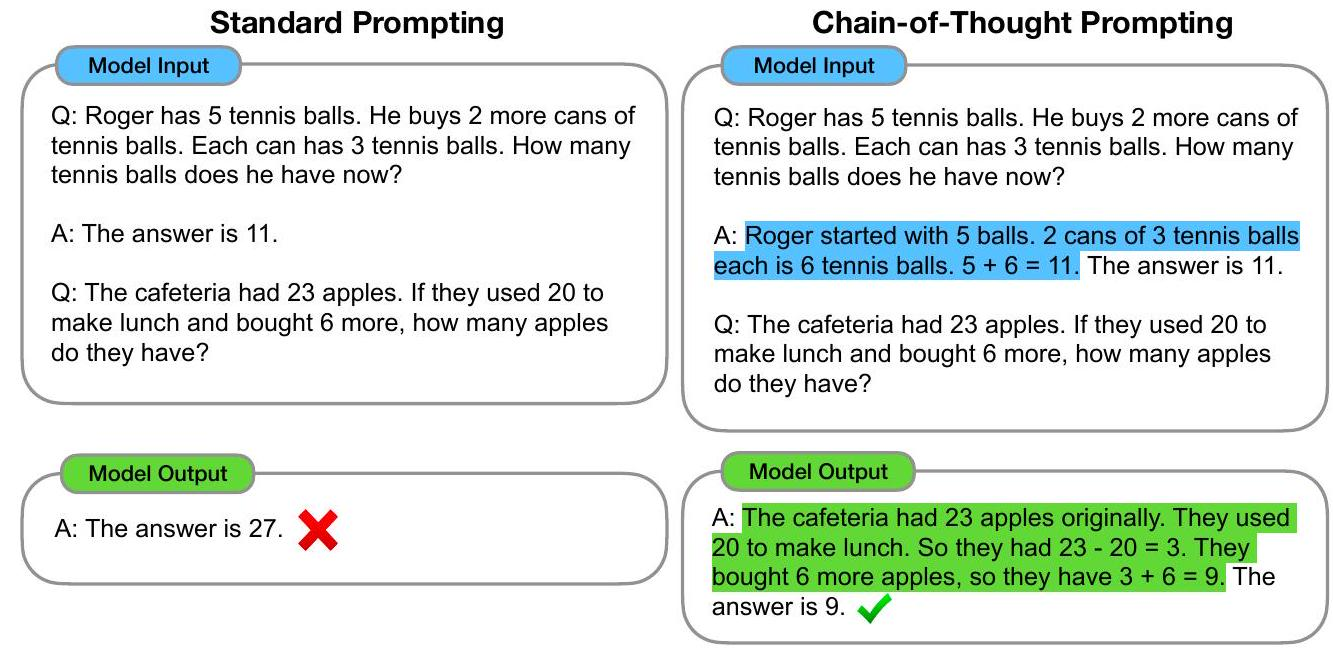
\includegraphics[width=0.75\textwidth]{img/cot_prompting}
        \captionsetup{font=small,labelformat=empty}
        \caption{Chain-of-Thought reasoning processes are highlighted.}
    \end{figure}
\end{frame}

\begin{frame}{CoT Techniques}
    \begin{figure}[!htb]
        \centering
        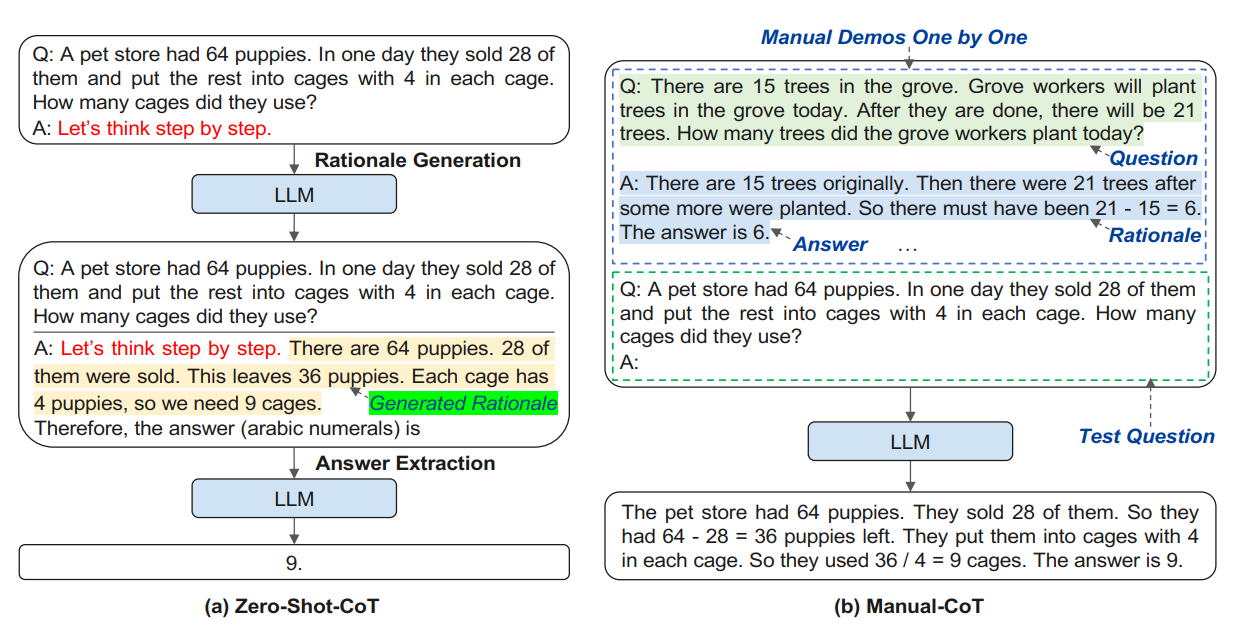
\includegraphics[width=\textwidth]{img/cot_types}
        \captionsetup{font=small,labelformat=empty}
        \caption{Zero-shot-CoT vs. Manual-CoT.}
    \end{figure}
\end{frame}

\begin{frame}{CoT Techniques}
    An automatic CoT prompting method (Auto-CoT~\cite{zhang2022automatic}), generates diverse samples and reasoning chains. In ten GPT-3 benchmark reasoning tasks, it consistently meets or surpasses manual CoT performance.
    \begin{figure}[!htb]
        \centering
        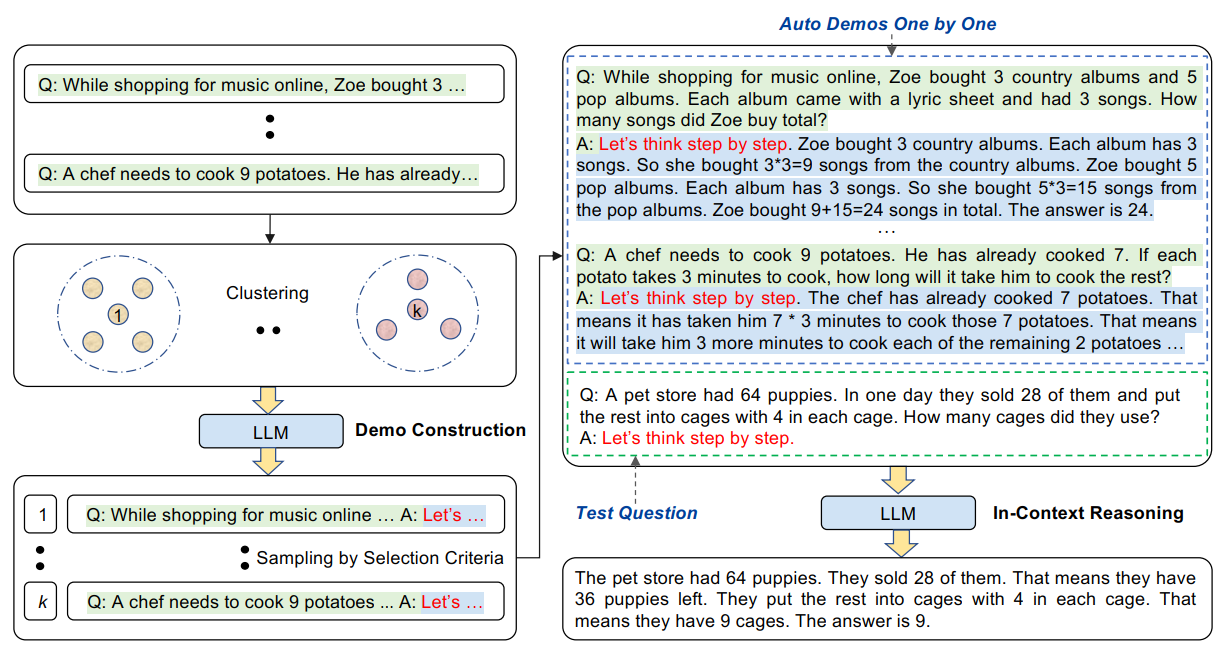
\includegraphics[width=0.85\textwidth]{img/auto_cot}
        \captionsetup{font=small,labelformat=empty}
        \caption{Auto-CoT.}
    \end{figure}
\end{frame}

\begin{frame}{CoT-SelfEvolve Architecture}
    \begin{figure}[!htb]
        \centering
        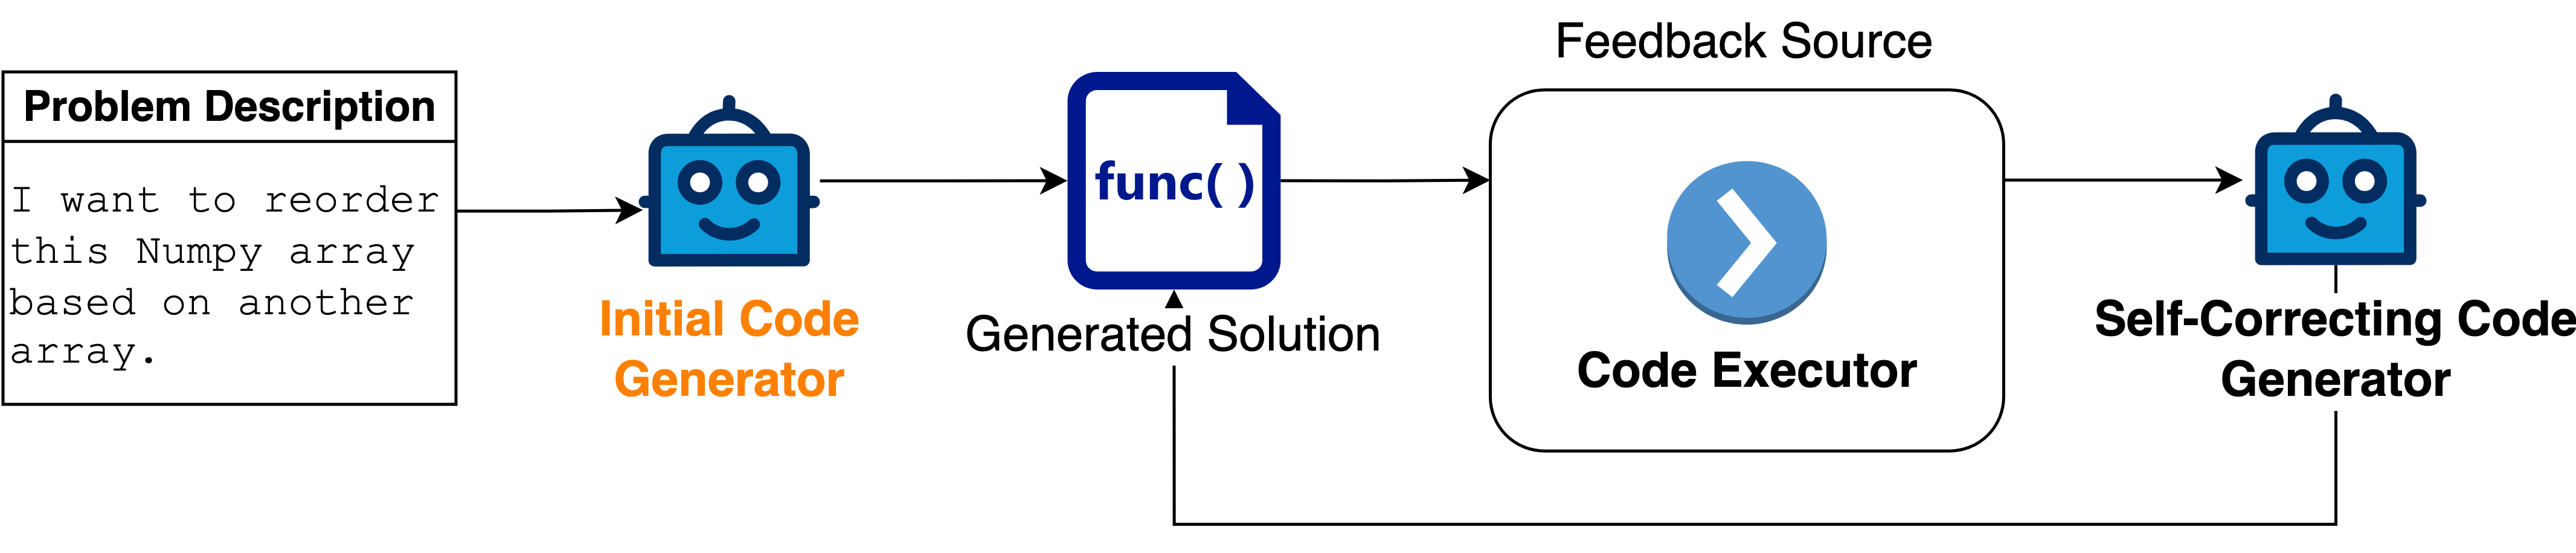
\includegraphics[width=0.70\textwidth]{img/selfevolve_architecture}
        \captionsetup{font=small,labelformat=empty}
        \caption{Architecture of the SelfEvolve~\cite{jiang2023selfevolve} model.}
    \end{figure}
    \begin{figure}[!htb]
        \centering
        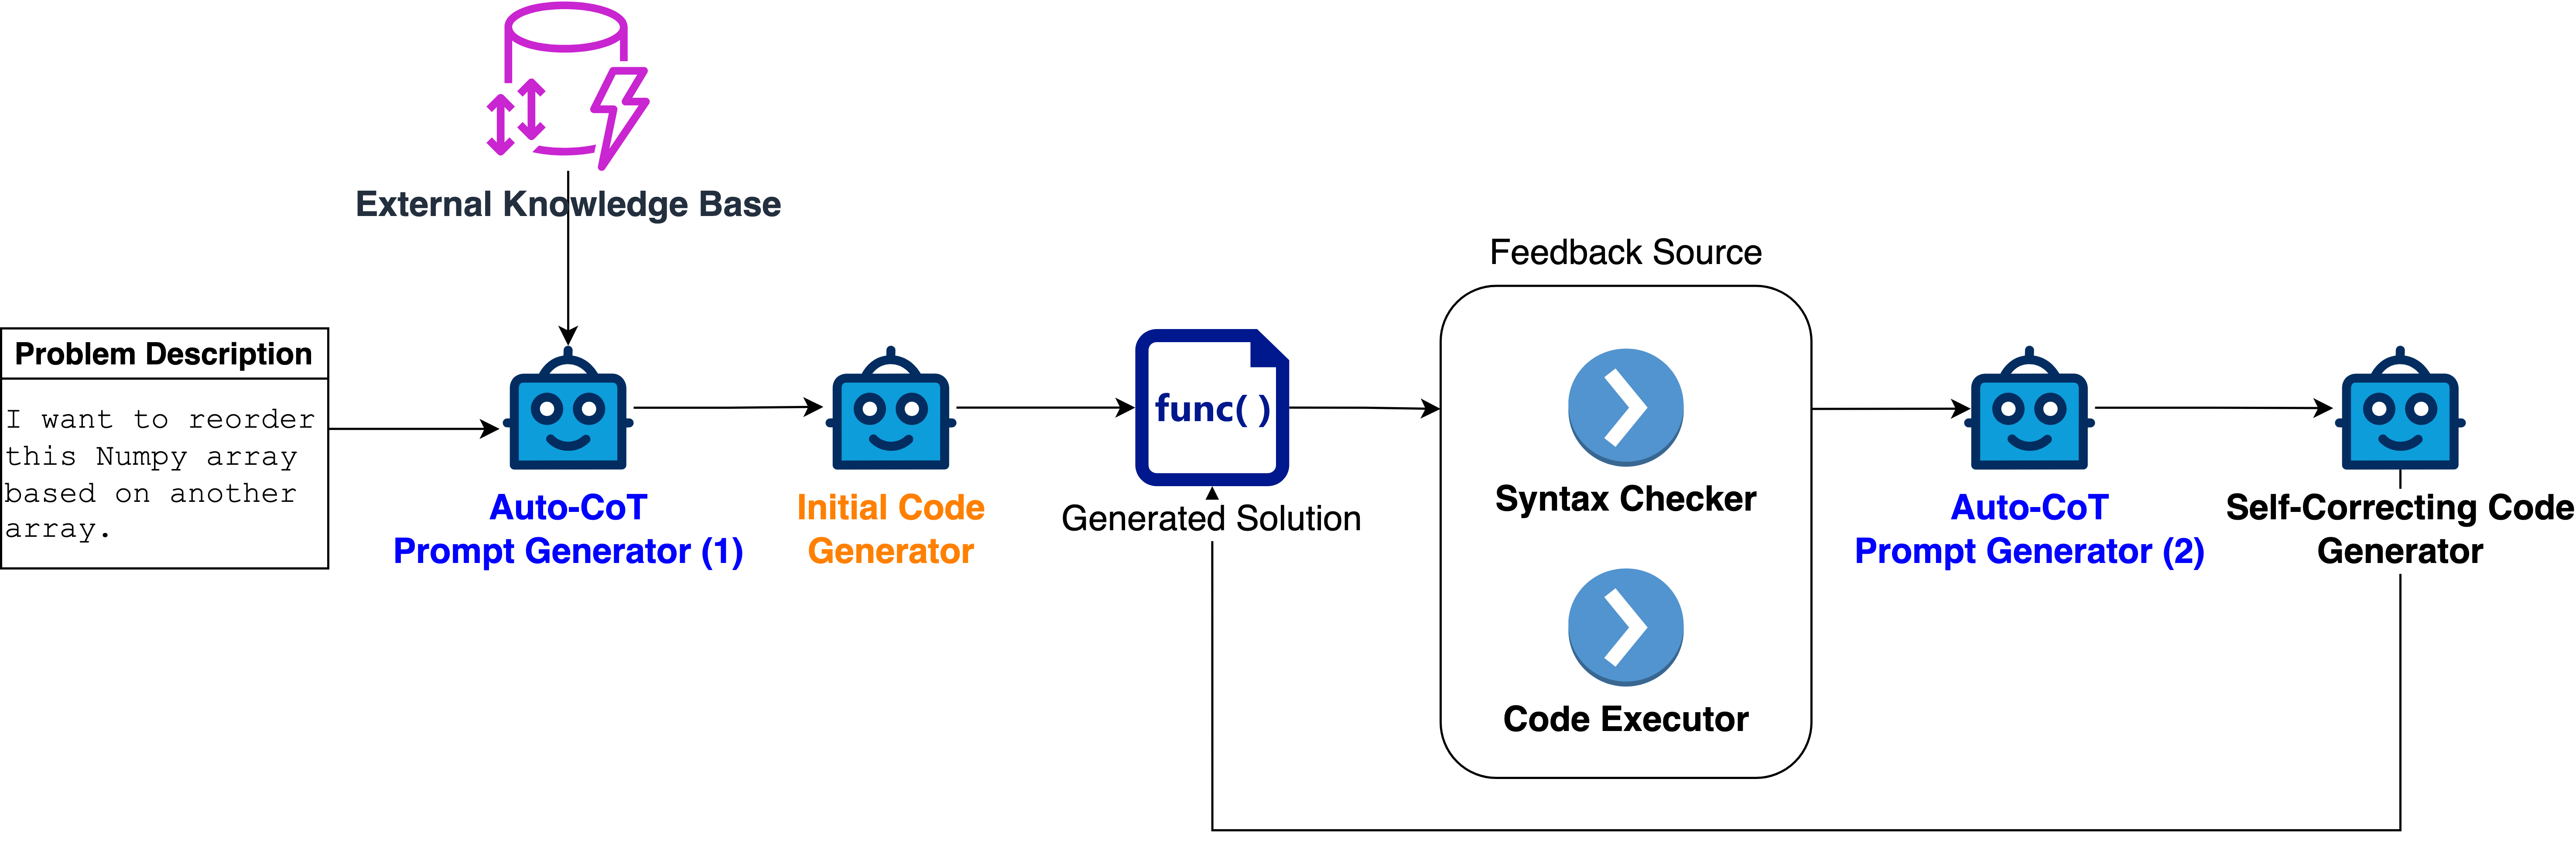
\includegraphics[width=0.90\textwidth]{img/cot_selfevolve_architecture}
        \captionsetup{font=small,labelformat=empty}
        \caption{Architecture of the CoT-SelfEvolve model (this study).}
    \end{figure}
\end{frame}

\begin{frame}{Auto-CoT Prompt Generation (1)}
    The initial Auto-CoT prompt generator integrates problem descriptions with relevant StackOverflow discussions. This in-context material aids a LLM in reasoning and hint generation for problem-solving. These hints then serve as CoT prompts for another LLM (Code Generator).
    \begin{figure}[!htb]
        \centering
        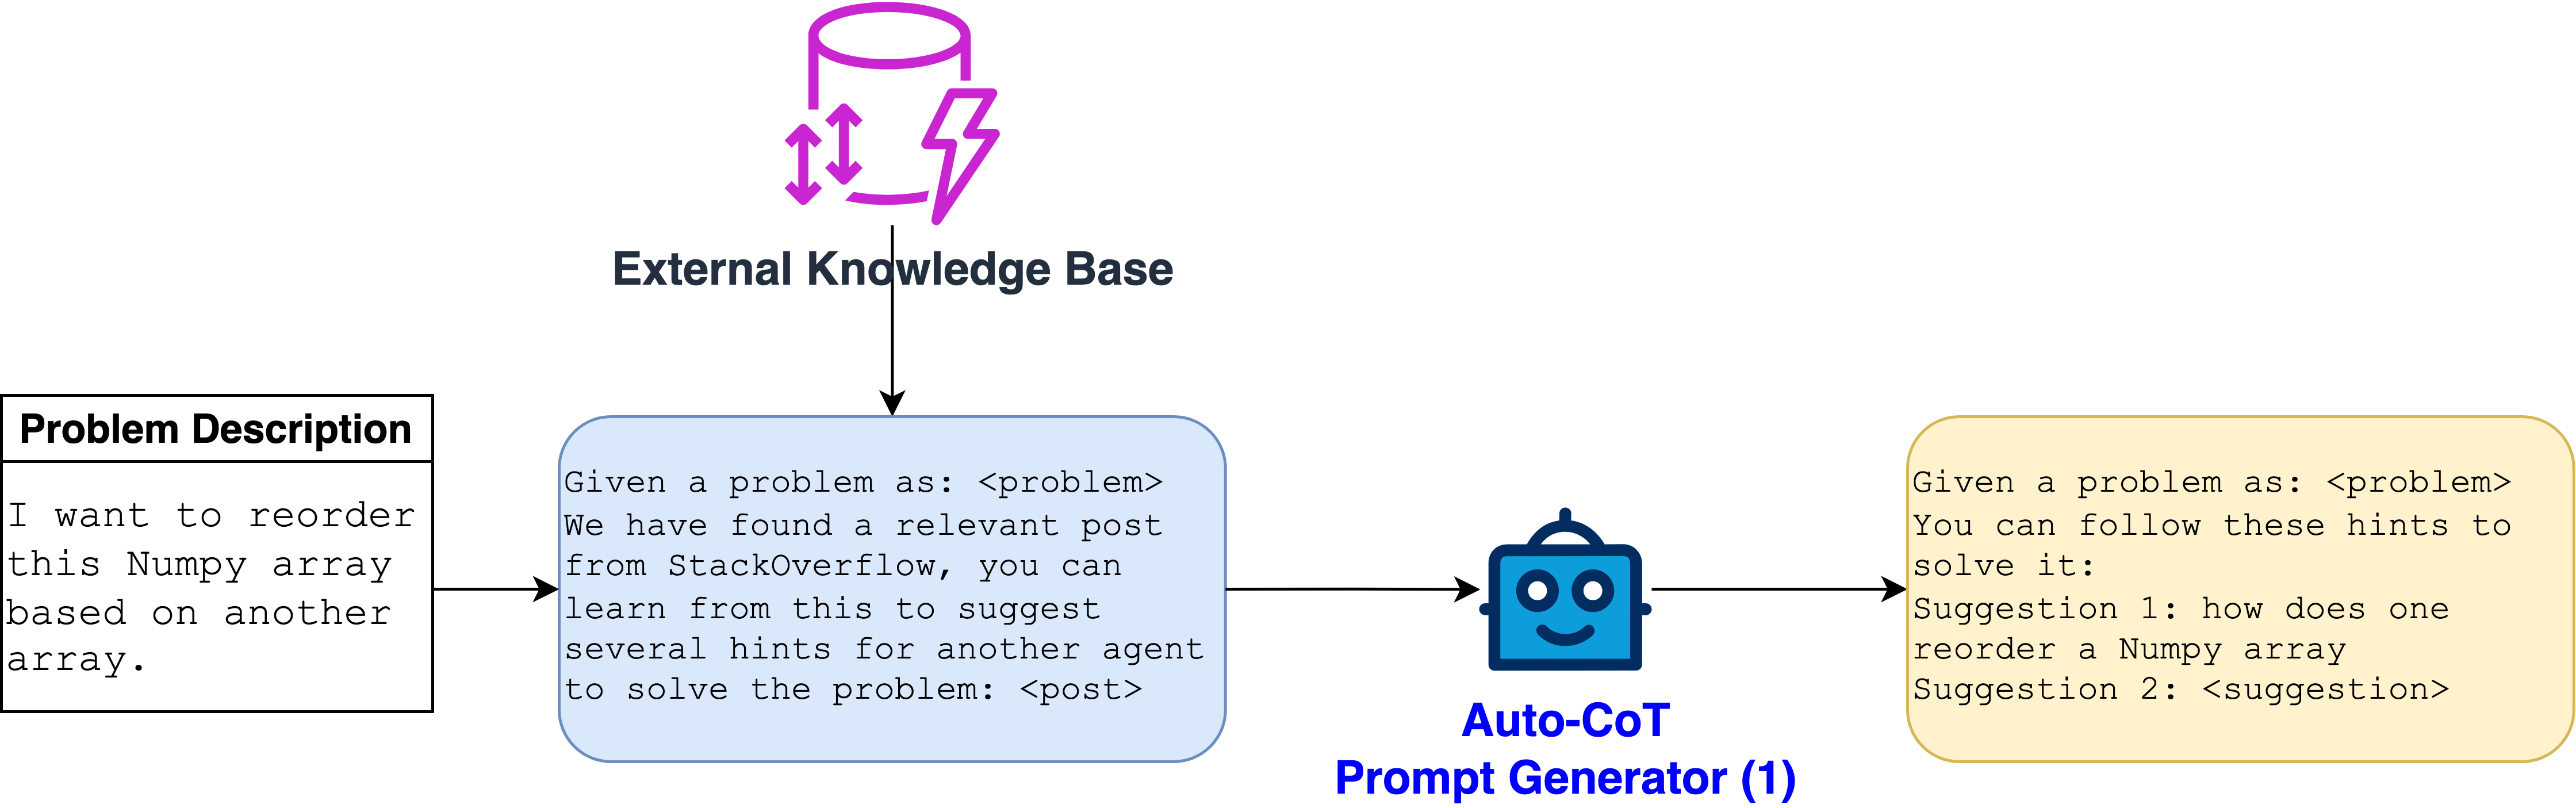
\includegraphics[width=\textwidth]{img/cot_generator_1}
        \captionsetup{font=small,labelformat=empty}
        \caption{Auto-CoT Prompt Generation (1).}
    \end{figure}
\end{frame}

\begin{frame}{Auto-CoT Prompt Generation (2)}
    The second Auto-CoT prompt generator combines problem descriptions with feedback from syntax checkers or code executors. It aims to generate self-reflective questions for a LLM to consider during problem-solving.
    \begin{figure}[!htb]
        \centering
        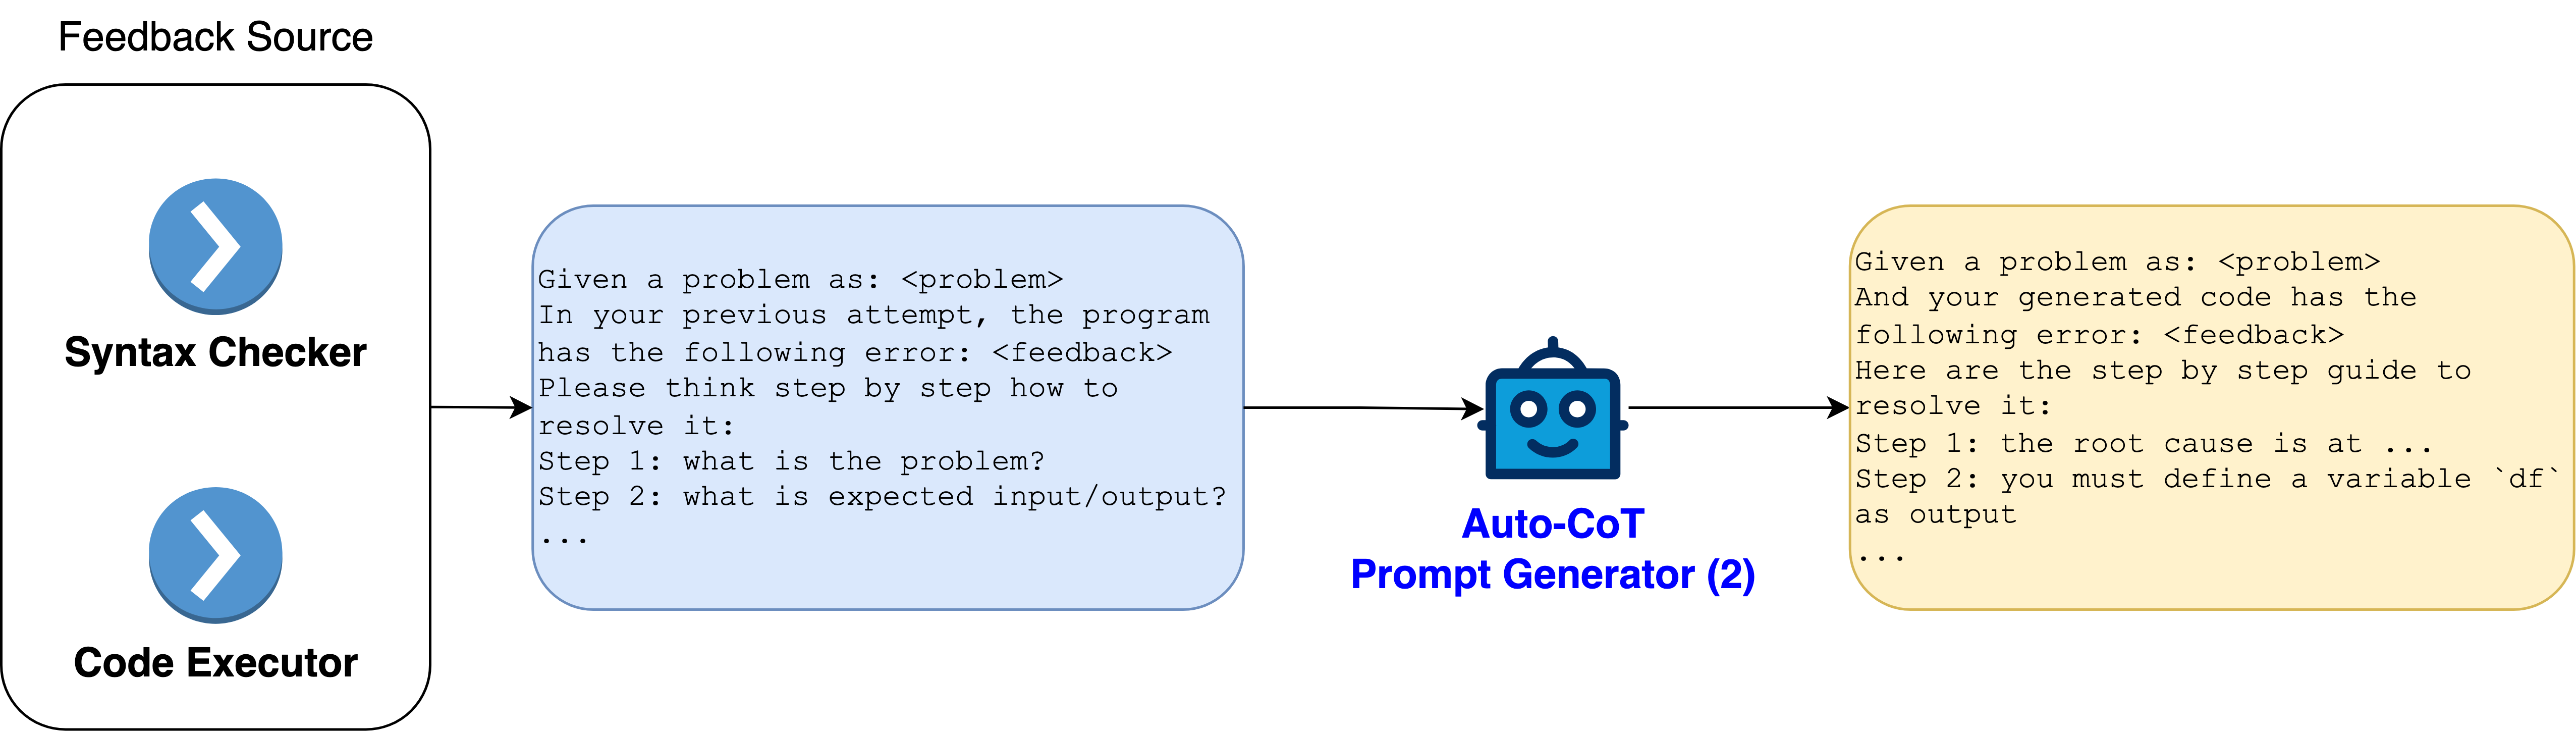
\includegraphics[width=\textwidth]{img/cot_generator_2}
        \captionsetup{font=small,labelformat=empty}
        \caption{Auto-CoT Prompt Generation (2).}
    \end{figure}
\end{frame}

\begin{frame}{External Knowledge Base}
    \begin{columns}[T] % align columns
        \begin{column}{.4\textwidth}
            \begin{figure}[!htb]
                \centering
                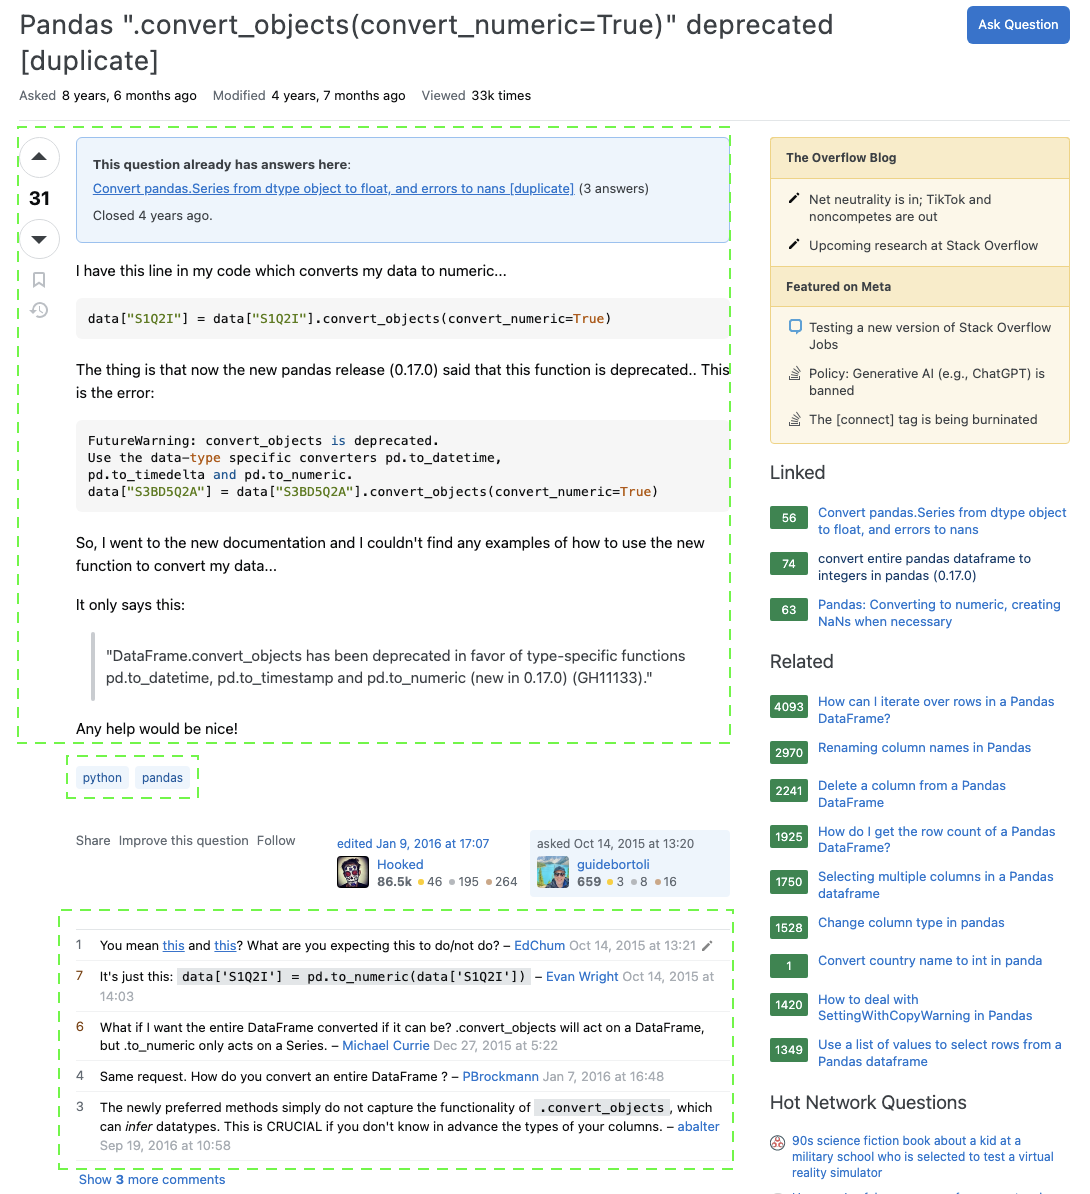
\includegraphics[width=\textwidth]{img/stackoverflow.png}
                \captionsetup{font=small,labelformat=empty}
                \caption{Example of StackOverflow discussions.}
            \end{figure}
        \end{column}%
        \begin{column}{.6\textwidth}
            \begin{itemize}
                \item An external knowledge base, narrowed to seven Python libraries, is constructed from 500,000 StackOverflow discussions.
                \item Each document amalgamates a problem description with its comments.
                \item OpenAI's text-embedding-ada-02 model generates the embeddings.
                \item Using the HNSW algorithm on top of these embeddings to retrieve relevant documents for a specific problem.
            \end{itemize}
        \end{column}%
    \end{columns}
\end{frame}
